% !TEX spellcheck = en_US
% !TEX encoding = UTF-8

\documentclass[a4paper, 12pt]{article}

\usepackage{scrextend}
\usepackage{graphicx}
\usepackage[tuenc]{fontspec}
\usepackage{xcolor}

% \usepackage[hidelinks, urlcolor=blue]{hyperref}
\usepackage[
  colorlinks=true,
  linkcolor={red!30!black},
  citecolor={blue!50!black},
  urlcolor={blue!80!black}
]{hyperref}
\usepackage{csquotes}
\usepackage[british]{babel}
\usepackage[backend=biber, sorting=none, dateabbrev=false]{biblatex}

\usepackage[bindingoffset=1.5cm, textwidth=15cm]{geometry}

\usepackage{tikz}
\usepackage{amsmath, amsfonts, amssymb}

\usepackage{pgfgantt}
\usepackage{subcaption}
\usepackage{float}
\usepackage{array}
\usepackage{enumitem}
\usepackage{multirow}
\usepackage{makecell}
\usepackage{hhline}
\usepackage{fixfoot}
\usepackage{bm}
\usepackage[acronym, toc, numberline]{glossaries}
\usepackage[format=plain,
            labelfont={bf,it},
            textfont=it]{caption}
% TODO: Fix caption

\usetikzlibrary{positioning}

\setmainfont{CMU Serif}
\setlength{\parskip}{\baselineskip}

\newcolumntype{P}[1]{>{\raggedright\arraybackslash}p{#1}}

% Fix bibliography parameters for overfull
\setcounter{biburlnumpenalty}{5000}
\setcounter{biburllcpenalty}{7000}
\setcounter{biburlucpenalty}{8000}

% Bibliography
\addbibresource{../bibliography/mendeley.bib}

\newcommand{\secc}{\ifdef{\chapter}{\chapter}{\section}}
\newcommand{\ssecc}{\ifdef{\chapter}{\section}{\subsection}}
\newcommand{\sssecc}{\ifdef{\chapter}{\subsection}{\subsubsection}}

\newcommand{\seccn}{\ifdef{\chapter}{chapter}{section}}
\newcommand{\sseccn}{\ifdef{\chapter}{section}{subsection}}
\newcommand{\ssseccn}{\ifdef{\chapter}{subsection}{subsubsection}}

\newcommand{\addphantomsec}[2]{%
  \cleardoublepage
  \phantomsection
  \addcontentsline{toc}{#2}{\numberline{}#1}
  \secc*{#1}
}

% Reduce the table of contents length
\makeatletter
\pretocmd{\secc}{\addtocontents{toc}{\protect\addvspace{15\p@}}}{}{}
\pretocmd{\ssecc}{\addtocontents{toc}{\protect\addvspace{-5\p@}}}{}{}
\pretocmd{\sssecc}{\addtocontents{toc}{\protect\addvspace{-9\p@}}}{}{}
\makeatother

% !TEX root = main.tex

\makeglossaries

\newglossaryentry{test}{
  name=test,
  description={
    This is just a test
  }
}

\newglossaryentry{censoring}{
  name=censoring,
  description={
    If a subject does not have an event during the observation time, they are described as
    censored. This means that nothing is known about the subject after the censoring
  }
}

\newglossaryentry{baseline}{
  name={baseline data},
  symbol={\( x \)},
  description={
    Available data to predict the survival time
  }
}

\newglossaryentry{time}{
  name=time,
  symbol={\( T \)},
  description={
    Time from the beginning of the observation period until an event, the end of the study
    or withdrawal from the study
  }
}

\newglossaryentry{event}{
  name=event,
  symbol={\( E \)},
  description={
    It can be death (\( E = 1 \)) or, otherwise, it can be recovery or withdrawal \( E = 0 \)
  }
}

\newacronym{UPC}{UPC}{Universitat Politècnica de Catalunya}
\newacronym{CFIS}{CFIS}{Centre de Formació Interdisciplinari Superior}
\newacronym{FIB}{FIB}{Facultat d'Informàtica de Barcelona}
\newacronym{CNN}{CNN}{Con\-vo\-lu\-tio\-nal Neural Networks}
\newacronym{MRI}{MRI}{Magnetic Resonance Imaging}
\newacronym{PET}{PET}{Positron Emission Tomography}
\newacronym{CT}{CT}{Computed Tomography}
\newacronym{CI}{CI}{Concordance Index}
\newacronym{ROC}{ROC}{Receiver Operating Characteristics}
\newacronym{OPSCC}{OPSCC}{Oropharyngeal Squamous Cell Carcinoma}
\newacronym{HNSCC}{HNSCC}{Head and Neck Squamous Cell Carcinoma}
\newacronym{CPH}{CPH}{Cox Proportional Hazards}
\newacronym{PMHNK}{PMHNK}{Princess Margaret Head and Neck}
\newacronym{DNN}{DNN}{Deep Neural Networks}



%%%%%%%%%%%% BEGIN OF DOCUMENT %%%%%%%%%%%%%%%%%%
\begin{document}

% Title page can be commented to remove it
\begin{titlepage}
  \centering
  \vspace{1.5cm}
  {\huge \textbf{\textsc{Unlock the potential of medical imaging data using deep learning}} \par}
  \vspace{1cm}
  {\Large \textit{Joan Marcè i Igual}\par}
  \vfill
  {Director: Dr.~Benjamin \textsc{Haibe-Kains} \par}
  {Tutor: Dr.~Maria José \textsc{Serna Iglesias} \par}
    
  \vfill

  
\includegraphics[width=0.3\textwidth]{images/logo_FIB}\par
  
  \vspace{.2cm}
  
  
\includegraphics[width=0.2\textwidth]{images/logo_upc}\par
  
  \vfill
  
  % Bottom of the page
  {\Large Computer Science Specialization \par}
  {\LARGE Facultat d'Informàtica de Barcelona \par}
  {\LARGE Universitat Politècnica de Catalunya \par}
  {\LARGE 2018 \par}
\end{titlepage}

\tableofcontents

\cleardoublepage
\phantomsection
\addcontentsline{toc}{\seccn}{\numberline{}List of Figures}
\listoffigures

\cleardoublepage
\phantomsection
\addcontentsline{toc}{\seccn}{\numberline{}List of Tables}
\listoftables

\pagebreak

% Just comment this lines to enable/disable some parts of the document
% !TEX root = main.tex

\secc{Context and scope of the project}
\ssecc{Context}

Nowadays one of the most extensive uses of computing is artificial intelligence. A few 
examples are Amazon purchase recommendations, based on previous purchases, or help users
to interact with their phone by only using voice commands like Google Assistant. 
~\cites{neural:amazon}{neural:google-assistant}

Inside AI one of the domains that has greatly increased during the last years is 
\emph{Machine Learning}. The main advantage is that it can solely learn from examples without 
explicit teaching, and thus reducing the human interaction during the learning process. One of the 
most used types is \emph{deep neural networks} and these have demonstrated impressive performance 
against computer vision and Natural Language Processing tasks like the classification of 
digits from the MNIST data set.
~\cites{neural:mnist}{neural:empirical-evaluation-deep-architectures}

Regarding the medical field, recent deep learning algorithms, specially \gls{CNN} 
have started to push the boundaries of precision medicine. 
Traditionally, medical predictions have been based on a few clinical parameters with poor accuracy.
However, other data types are available to improve such predictions. In this context, medical
images generated from \gls{MRI}, \gls{PET} or \gls{CT} scans are vastly underused 
due to the 
inability of radiologists to quantitatively analyze this complex data.

Different methods have appeared to analyze these images for tasks such as
image classification, object detection, segmentation and registration among other tasks. This
approach started in the late 1990s and has slowly shifted from systems that are completely designed
by humans to systems that are trained by computers using example data. 
~\cite{medical:survey-deep-learning}

Professor Benjamin Haibe-Kains has helped in the development of \emph{Radiomics}, a new field to
relying on pre-defined, hand-engineered features computed from medical images to better 
characterize tumours and predict survival outcome. Although promising, radiomics suffers from 
several limitations. The most important one is that it relies on hand-engineered features,
these features are not guaranteed to be the most discriminant ones. Deep learning methods
are end-to-end and, for a given task, they drive features from the data.
~\cite{medical:radiomics-ml-classifiers}

\sssecc{Survival Analysis}

Survival Analysis is a branch of statistics that analyzes the duration time of the observed
events. Typically it refers to the time to the failure of a physical component or to death of a
patient. It usually defines the following terms~\cite{neural:survival-analysis}:

\begin{description}
  \item[\Gls{event} \glssymbol{event}] \glsdesc{event}
  \item[\Gls{time} \glssymbol{time}] \glsdesc{time}
  \item[\Gls{baseline} \glssymbol{baseline}] \glsdesc{baseline}
  \item[\Gls{censoring}] \glsdesc{censoring}
\end{description}

The survival and hazard functions are the two fundamental functions in survival analysis. The
survival function \( S(t) = \Pr(T \ge t) \), is the probability that an individual has
\emph{survived} beyond time \( t \). The hazard function \( \lambda(t) \) is a measure of risk at 
time \( t \) and it's defined as:
~\cite{medical:cox}
\[
  \lambda(t) = \lim_{\Delta t \rightarrow 0}
  \frac{\Pr(t \le T < t + \Delta t | T \ge t)}{\Delta t}
\]

Usually, when trying to fit a survival model a \gls{CPH} model is used. This type of model
intends to use the \gls{baseline} \( \bm{x} = (x_1, x_2, ..., x_p) \)
to fit the hazard function \( \lambda(t) \)
in the following way:
\[
  \lambda(t | \bm{x}) = \exp(\bm{x}\bm{\beta}) \cdot \lambda_0 (t)
\]
Where \( \bm{\beta} \) is a \( p \times 1 \) vector of unknown parameters, that need to be fit, 
and \( \lambda_0(t) \) is an unknown function giving the standard set of conditions 
\( \bm{x} = \bm{0} \). As it can be seen this model requires for a log-linear relation between
the \gls{baseline} \glssymbol{baseline} and the hazard function \( \lambda(t | \bm{x}) \).

However, casting the survival analysis as a ranking problem is a way of dealing with the biased
distributions of survival times and the censoring data. Two subjects' survival times can be 
ordered only if:
\begin{enumerate}[noitemsep, topsep=0pt]
  \item Both of them are uncensored (\( E_i = E_j = 1\))
  \item The uncensored time of one is smaller than the censored survival time of the other
  (\( T_i < T_j | E_i = 1; E_j = 0 \))
\end{enumerate}

This can be visualized by means of an order graph \( G = (V, E) \), see \autoref{fig:graph-ci}.
The set of vertices \( V \) represents all the individuals, where each filled circle 
(\( \bullet \)) indicates an \emph{uncensored} survival time, while an empty circle 
(\( \circ \)) denotes a \emph{censored} observation.
Existence of an edge \( E_{ij} \) implies that \( T_i < T_j \). An edge cannot originate 
from a censored point.

\begin{figure}
  \centering
  \begin{subfigure}[b]{.4\textwidth}
    \centering
    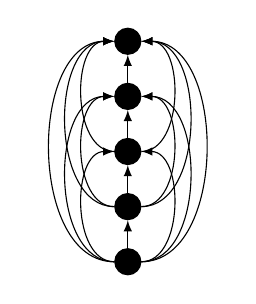
\begin{tikzpicture}[scale=.7]
  \tikzstyle{bDot}=[circle, fill=black, draw]
  \foreach \y in {1,...,5} {
    \node[bDot] (D-\y) at (0, \y) {};
  }

  \foreach \y in {1,...,4} {
    \pgfmathsetmacro{\z}{int(\y + 1)}
    \draw[-latex] (D-\y) -- ({D-\z}.south);
  }

  \foreach \y in {1,...,3} {
    \pgfmathsetmacro{\z}{int(\y + 2)}
    \foreach \j in {\z,...,5} {
      \ifthenelse{\y=2 \OR \y=3}{
        \draw[-latex] (D-\y) to[bend left=90] (D-\j);
      }{
        \draw[-latex] (D-\y) to[bend right=90] (D-\j);
      }
    }
  }
\end{tikzpicture}

    \caption{Without censored data}
  \end{subfigure}
  ~
  \begin{subfigure}[b]{.4\textwidth}
    \centering
    \begin{tikzpicture}
  \foreach \y in {1,...,5} {
    \ifthenelse{\y=2 \OR \y=4}{
      \node [circle, fill=white, draw=black] (D-\y) at (0, \y) {};
    }{
      \node [circle, fill=black, draw=black] (D-\y) at (0, \y) {};
    }

    \foreach \y in {3,4,5} {
      \draw [-latex] (D-1) to[bend right=90] (D-\y);
    }

    \foreach \y/\z in {1/2, 3/4} {
      \draw [-latex] (D-\y) -- (D-\z);
    }
    \draw [-latex] (D-3) to[bend left=90] (D-5);
  }
\end{tikzpicture}

    \caption{With censored data}
    \label{fig:graph-ci:censored}
  \end{subfigure}

  \caption{Order graphs representing the ranking constraints \label{fig:graph-ci}}

  Censored data is represented by \( \circ \) and uncensored data is represented by \( \bullet \).
  Every edge \( A \rightarrow B \) means \( T_A > T_B \). Note that in 
  \autoref{fig:graph-ci:censored} some vertex are not connected since an edge 
  \( \circ \rightarrow \bullet \) cannot be formed.
\end{figure}

% C-index explanation
The standard performance measure, to compare if a survival 
model is performing better than another, is the \gls{CI}. To obtain this 
indicator, pairs are generated to compare the survival time. A prediction is counted as good only
if both \( T_i > T_j \) and \( \hat{T}_i > \hat{T}_j \), otherwise
it's counted as a bad prediction, note that \( T_i = \hat{T}_i \) it's not a required condition. 
Then, the number of good predictions is divided by the total predictions. 
~\cite{medical:ranking-ci}

\[
  CI = \frac{\text{Good predictions}}{\text{Total predictions}} \in [0, 1]
\]

Also, another comparison 
element is the \gls{ROC} curve which represents the \emph{False Positive Rate} against the 
\emph{True Positive Rate}, see \autoref{fig:ROC-curve}. Usually the \gls{CI} is seen as 
the area under the \gls{ROC} curve.
~\cite{neural:roc-precision-recall}

\begin{figure}
  \centering
  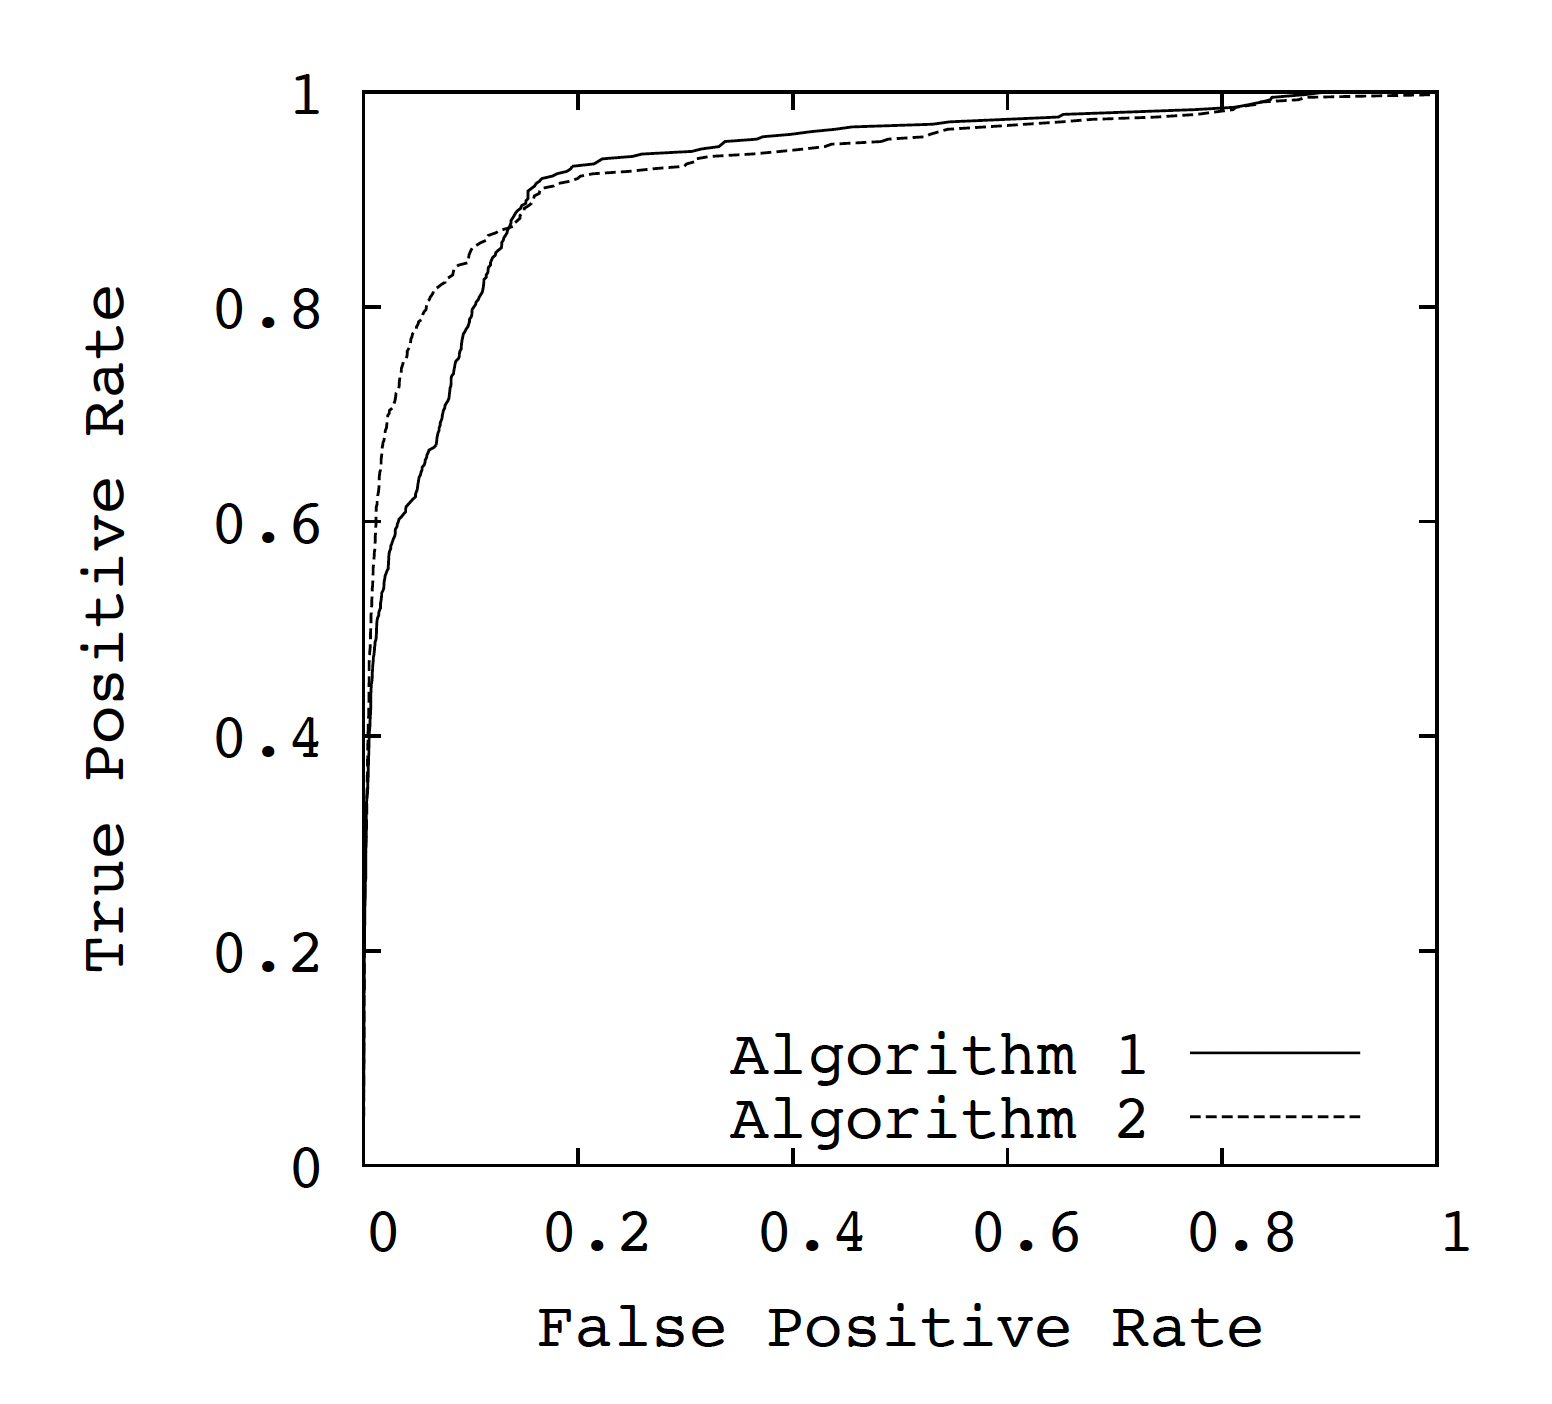
\includegraphics[width=.5\linewidth]{images/roc_curve}
  \caption{\acrshort{ROC} Curve example\label{fig:ROC-curve}}
\end{figure}

\sssecc{Dataset}

The dataset used by this project to develop a model is provided through a 
collaboration with Dr.~Fei-Fei Liu, head of the Radiation Medicine Program at Princess
Margaret Cancer Centre.

We have access to a unique set of 671 cancer patients diagnosed of \gls{OPSCC}. Accounting
for approximately half a million cases annually worldwide, \gls{HNSCC} 
is a considerable cause of mortality and morbidity, with the majority of patients having
locally advanced, unresectable disease. \gls{OPSCC} has been one of the fastest growing 
disease sites for \gls{HNSCC}.
~\cite{medical:ct-based-radiomic-signature}

Multiple information is provided for each patient. There's a \gls{CT} scan where the tumour 
can be seen clinical information about the patient. The scan is 512 pixels wide by 512 
pixels tall and is composed of 100-200 slices in gray scale that together form a 3D image. 
To be able to slice the tumour from the rest of the image, a mask of the same size as the scan 
is provided. The masks contains information about the tumour location, it has \texttt{1}s 
in the pixels containing the tumour and \texttt{0}s
otherwise, as it can be seen in \autoref{fig:dataset-example}.

In the following document we will be calling this the \gls{PMHNK} dataset.

Regarding the clinical information the following fields are provided:
\begin{itemize}
  \item Subject characteristics (age, gender, clinical status, smoking, drinking history)
  \item Tumor characteristics (cancer location, staging, p16 status)
  \item Treatment data (modality, radiation start/end dates, radiation dose/fractionation, 
  treatment completion status)
  \item Outcome data (status, cause of death, local failure, regional failure, distant failure)
\end{itemize}

\begin{figure}
  \centering
  \begin{subfigure}[t]{.32\textwidth}
    \centering
    
\includegraphics[width=\textwidth]{images/IMG_example.png}
    \caption{Original image}
  \end{subfigure}
  \hfill
  \begin{subfigure}[t]{.32\textwidth}
    \centering
    
\includegraphics[width=\textwidth]{images/IMG_MASS_example.png}
    \caption{Image mask}
  \end{subfigure}
  \hfill
  \begin{subfigure}[t]{.32\textwidth}
    \centering
    
\includegraphics[width=\textwidth]{images/IMG_merge_example.png}
    \caption{Mask applied to original}
  \end{subfigure}

  \caption{Example of images from the dataset \label{fig:dataset-example}}

  Single \gls{CT}'s scan slice, a whole scan is composed of multiple slices. By applying 
  the mask to the original image, the part that only contains the tumour can be extracted.
\end{figure}


\ssecc{State-of-the-art}

Nowadays, a lot of research is being done in the medical field using deep learning. Image
classification is one of the first areas in which there's a major contribution to medical analysis.
Usually in image classification there are one or multiple images as input and a single diagnostic 
variable as output (e.g.~ill or not).
~\cite{medical:survey-deep-learning}

Regarding the prediction of survival models, there have been different approaches although
almost all of them use \gls{MRI}, \gls{PET} or \gls{CT} scans and the clinical data. 
The typical one, is to extract hand-crafted radiomic features using own methods or using 
libraries such as \emph{PyRadiomics}. This 
hand-crafted features are usually based in aspects like tumour shape, intensity, volume or texture.
~\cites{medical:tumour-radiomics}{medical:py-radiomics}{medical:computational-radiomics}

An alternative approach, is to use a deep learning-based model for prediction and for feature
extraction. In this case, features are extracted too but a \gls{CNN} 
is used instead. With this approach, the use of transfer learning has been a
great improvement. Also, pre-trained networks are used to reduce the requirement of large data
sets for deep network training. Usually, there are two possible strategies: 
\begin{itemize}[noitemsep, topsep=0pt]
  \item Using a pre-trained NN as a feature extractor
  \item Fine-tuning a pre-trained network on medical data.
\end{itemize}

Both strategies are popular and have been widely applied. A network that allows this type
of retrain is GoogLeNet Inception v3
~\cites{neural:goog-le-net}{neural:retrain}{neural:inception-retrain}.
However, there's the added problem that medical imaging data are usually 3D images but, 
when working with pre-trained \gls{CNN}, only 2D images can be used, because there are still no 
pre-trained networks on 3D images. Although this method seems promising, still requires 
further work to train a dedicated feature extractor explicitly designed for medical images.
~\cite{medical:deep-learning-radiomics-gbm}

An implemented survival prediction model is \emph{DeepSurv} which is based on survival data
and uses the \gls{CPH} model for an individual's survival given the \gls{baseline}
\( x \). It's an Open Source Python module that applies recent deep learning techniques 
to a Cox model.
~\cites{medical:deep-surv}{medical:cox}

In the 3D imaging field, there has been some work too. 3D \glspl{CNN} have
been used for brain lesion segmentation on multi-channel \gls{MRI} scans. In this case a 
dual pathway of 11-layers deep 3D \gls{CNN} was used and was able to improve the previous
state-of-the art, the model structure can be seen in \autoref{fig:deepmedic} and the code 
can be found on GitHub. 
One of the biggest handicaps found was the computational intensity of
processing 3D medical scans, since they usually need a lot of memory and GPU time.
~\cites{neural:deepmedic}{neural:3d-cnn-crf}

\begin{figure}
  \centering
  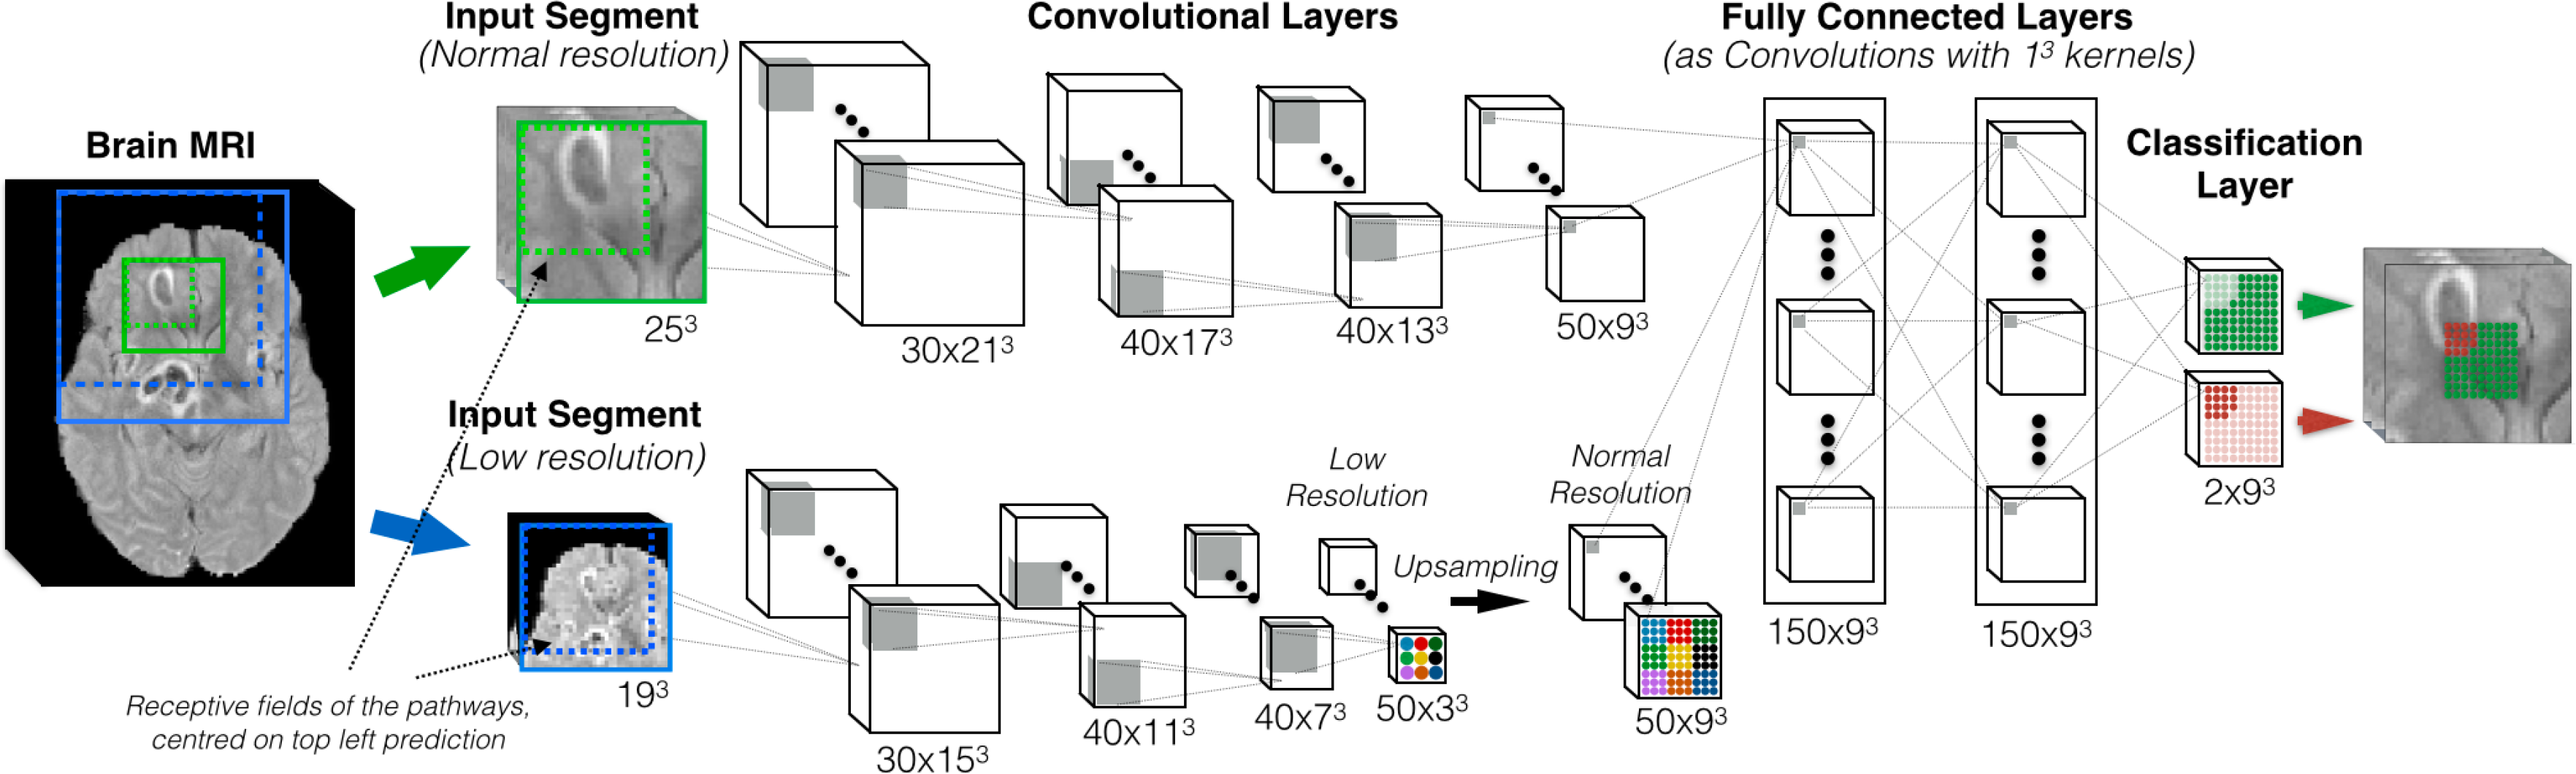
\includegraphics[width=\textwidth]{images/deepmedic}

  \caption{DeepMedic 3D \acrshort{CNN} model for brain lesion segmentation \cite{neural:3d-cnn-crf}
  \label{fig:deepmedic}
  }
\end{figure}

Another application of 3D \glspl{CNN} has been in action detection and segmentation for videos.
In this case video imaging was treated as a 3D image where the 3rd dimension represents
time.
~\cite{neural:3d-cnn-action-detection}

On the \gls{PMHNK} dataset some results have already been obtained. By using the \gls{CT} scans and
extracting some features. In this case, the extracted features were:
\begin{itemize}
  \item First order statistics: Energy
  \item Shape: Compactness
  \item Gray level run length: Gray level non-uniformity
  \item Wavelet (HLH) 
\end{itemize}
By fitting the features through a \gls{CPH} model a \gls{CI} of 0.628 was obtained for the whole
dataset.
~\cite{medical:ct-based-radiomic-signature}

\ssecc{Problem Formulation}

This problem is centered around survival prediction and it will be using the \gls{PMHNK} dataset. 
As it has been previously said, the current results for the dataset is a \gls{CI}
of 0.628 \cite{medical:ct-based-radiomic-signature} by using four different features.

The problem statement will be as follows:
\begin{quotation}
  Can a better survival prediction than the current results, be obtained using imaging data and
  \gls{DNN}?
\end{quotation}

\ssecc{Objectives}

The objectives to achieve will be:
\begin{itemize}
  \item Get a better understanding of survival prediction problems.
  \item Be able to analyze the \gls{PMHNK} dataset to get different strategies for building a 
  deep learning model.
  \item Develop a new deep learning model to improve the survival's prediction rate for the
  \gls{PMHNK} dataset patients' compared to models built on traditional radiomic features.
  \item Investigate and compare the performance of the deep learning-based method to 
  the more conventional methods, such as hand-engineered radiomic features.
  \item Get a better \gls{CI} than the \emph{volume} feature, which is often used in clinic as a
  prognostic feature, its \gls{CI} is ~0.65.
\end{itemize}

\ssecc{Stakeholders}

\sssecc{Developer}
Is the person in charge of the research, document and implement all the required software.
In addition he is responsible for the project management and the writing of the report
and all the required documentation. This actor works as agreed with the director and
he is, ultimately, the person in charge of accomplishing the deadlines.

\sssecc{Director}
The project will be directed by professor Benjamin Haibe-Kains, from the Bioinformatics 
and Computational Genomics Laboratory. He is the main responsible for guiding, giving 
advice and, in general, helping the developer.
His action is key to determine possible errors in the project, both in its proposal and 
execution.
~\cites{bhklab}.

\sssecc{Beneficiaries}
The project beneficiaries will depend on its outcome. If a more efficient model is found, the
beneficiaries will be the researchers trying to test a new cancer treatment method. Moreover,
the final patient will also be benefited because more modern research techniques will be used.

However, if a more efficient model is not found, the beneficiaries will be future researchers
trying to find the best model for survival analysis, since this would prove which 
methods do not work well for this problem.

\ssecc{Scope}

This project will be centered around the \gls{PMHNK} dataset. This dataset will be analyzed
and a model will be created accordingly.

Since the project aims to create a machine learning model, the first task will be to learn and 
to understand how Neural Networks work. Also, since the inputs will have imaging data, learning
how \gls{CNN} work will be necessary too, as they are really useful for analyzing imaging data. 
This way, I will have a fully understanding of the 
background that all these methods use to create models for survival prediction.

The following task will be to understand how survival prediction problems are approached. An
example of survival prediction is the \emph{DeepSurv} python package, so being able to set 
up, to run and to understand the package will give me a bit more of background in the problem.
However, \emph{DeepSurv} uses a \gls{CPH} model but in this case an attempt will be made to use
a different model, since a \gls{CPH} model is only valid under certain circumstances.
~\cites{medical:deep-surv-github}{medical:cox}

Afterwards, a deep learning model will be created, starting from zero but trying to use some
ideas from other completed projects. The model, unlike \emph{DeepSurv}, will not be using
the \gls{CPH} model. In this case, the approach will be to directly optimize the \gls{CI}
instead of get a better prediction of the hazard function \( \lambda(t) \) to optimize 
the \gls{CI}.

To directly optimize the \gls{CI} the comparison of two pairs will be predicted instead. So,
for a pair of two patients \( A \) and \( B \) the model should predict if \( T_A < T_B \),
where \( T \) stands for survival time. So the output should be \( 1 \) if the condition holds
\texttt{true} and \( 0 \) otherwise.

To do so, a siamese neural network will be used,
this type of networks are best suited to compare similarity between the inputs and is usually
used for tasks such as face recognition. Since it will be used to compare a pair's survival
time and not similarity, some changes should be made before using the network.

\ssecc{Methodology}

This project is part of a research project at Benjamin Haibe-Kains Bioinformatics and 
Computational Genomics Laboratory \cite{bhklab}. This means that every week there will be a 
laboratory meeting where different members will be presenting their progress and feedback will
be received accordingly. Once in a while this project's progress will be presented there.

Moreover, a weekly meeting with the Principal Investigator will be scheduled to discuss
the progress made. This weekly meeting should help in determining possible errors during the 
project's development and provide further guidance.

Also, since fitting a machine learning model is not a straightforward task, this means that 
it will require a process of trial and error until the proper solution is found. 
So, during this process, tasks will be assigned on a weekly basis with the objective to
improve the results from the previous ones.

\ssecc{Possible obstacles and solutions}

\sssecc{Training time}

Since this project involves \gls{CNN}, the training time can be a problem. 
The convolution operation is computationally expensive so, depending on the network, the 
training time can be of several days. Usually this type of networks are trained using 
GPUs since the convolution operation can be performed faster in this type of processor. 
Also, while just inferring the values does not require
much power, training needs a lot more power. 

To solve this problem, the training will be done at \gls{CC} a computing facility which 
has multiple computing clusters with GPUs.

\sssecc{Monitoring Tools}

The work will be done with the help of Git and GitHub. This tools will help monitoring
the project's evolution. The purpose of Git is to be able to do small revisions,
named commits, and to document all the different changes in the project. Also, it's 
prepared to allow multiple contributors in the same project. Moreover,
Git projects can be stored in a server, GitHub it's an online platform that allows
remote Git repositories. GitHub has integrated an issue system, a milestone system
and it's really integrated with Git's contributor system.
~\cites{tool:git}{tool:github}

\sssecc{Bugs}

Considering the software development process, it's no big surprise that it's really easy to
introduce bugs while writing or modifying the source code. To ensure no bugs are present,
some unit tests will be written to check if the model is still giving correct results.
However, this will be a difficult task since it's not easy to check whether a deep 
learning model is just overfitting or that it's giving wrong results.

\sssecc{Scheduling}

Although four months seems plenty of time, spending more time than estimated in a single task
can happen. To avoid this problem weekly meetings will be scheduled with my Principal Investigator
to see which is the best way to continue to keep on track.

\sssecc{Not enough data}

Since the starting dataset is quite small (\( \sim 500 \) samples) overfitting may be a problem
and different methods should be used to avoid it. The possible solutions are:
\begin{itemize}
  \item Using regularization to avoid units with a very high weight.
  \item Using dropout to force each unit to learn with only part of the data, and thus generalize.
  \item Using data augmentation techniques such as random crops or random rotations to increase
  the number of images in the dataset.
\end{itemize}

% !TEX root = main.tex


\section{Project Planning}

\subsection{Planning and scheduling}

The estimated project duration is of about 4 months. The project starts on Wednesday 14th of 
February, 2018 and the deadline is on Sunday 17th June, 2018, the week before the 
presentations start.

During the development of the project there will be weekly lab meetings with my Principal
Investigator, prof. Benjamin Haibe-Kains, where the development of the project will be 
discussed. There I should show my work done and how to approach each of the problems as
they appear.

Moreover, once a week, a lab meeting will be scheduled. Its objective will be to show
the development and improvements of different lab members and receive feedback from the 
members.

It must be noticed that the initial planning can be revised and updated as a result of the 
project's evolution, feedback received from the lab members and from my Principal Investigator. 

\subsection{Task description}

\subsubsection{Acquire background in Convolutional Neural Networks}

The first step is to acquire a better understanding in how a convolutional neural network works.
Therefore, in the las month I've been learning about Convolutional Neural Networks and how they
can be used. 
I started with basic statistics applied to \emph{Machine Learning} by reading the book 
\emph{The Elements of Statistical Learning}.~\cite{ElementsStatisticalLearning}

Then, I continued by doing three courses made by \href{https://www.deeplearning.ai}{Deeplearning.ai}
and published at Coursera~\cite{Coursera} related to Convolutional Neural Networks:
\begin{itemize}
  \item \href{https://www.coursera.org/learn/neural-networks-deep-learning}{Neural Networks and 
    Deep Learning}~\cite{Coursera:NN}: Where the basic elements of a neural network and how
    to train it are explained.

  \item \href{https://www.coursera.org/learn/deep-neural-network}{Improving Deep Neural Networks: 
    Hyperparameter tuning, Regularization and Optimization}~\cite{Coursera:NNHyperparameters}: 
    In this course it's shown the importance of hyperparameters and how each one works. 
    This way then it can be easier to design a proper network. Also, the different methods 
    of regularization are explained too, so overfitting can be avoided.

  \item \href{https://www.coursera.org/learn/convolutional-neural-networks}{Convolutional Neural 
    Networks}~\cite{Coursera:CNN}:
    How the \emph{convolution} operation works and why it's used in Machine Learning. 
    Different methods of using a Convolutional Neural Network, like face recognition or 
    object detection, are taught too.
\end{itemize}

All the tasks where done in three weeks.

\subsubsection{Get familiar with survival models like DeepSurv}

Survival Prediction models are a bit different from the typical Machine Learning problem. 
In this case, the desired output values are not the event indicator \( E \) and the time
interval \( T \). What we want to obtain is the survival function \( S(t) \) or the 
hazard function \( \lambda(t) \).

DeepSurv is one of the machine learning papers using a survival model, in this case the
Cox Proportional Hazards model which is not the same I will be planning to use.

To see how to properly use a survival model in a deep learning application i should fully 
understand how this is applied in the construction of the DeepSurv neural network. During 
the task I should compare the code implementation with the theoretical models so this way
I can see how to properly use \emph{vectorization} to speed-up computation
\cites{Cox}{DeepSurv}.

This process will take around two weeks.

\subsubsection{Preprocess data}

The input data for this project are:
\begin{itemize}
  \item RAW data from CT scans. There are around 88 slices for each patient, each one of 
  a size of \( 512 \times 512 \) pixels.
  \item Tumour annotations for the CT scans. For each RAW scan there's another slice which
  is a mask of 1s and 0s where the value is 1 if there's a tumour in that pixel.
  \item Clinical data. Which has information for each patient such as:
  \begin{itemize}
    \item Age
    \item Gender
    \item Smoking Pack Years
    \item Treatment
    \item Survival time
    \item Survival event
  \end{itemize}
\end{itemize}

All these data needs to be processed and for each CT scan, the 3D slice of the tumour needs to
be extracted and the pixel values need to be normalized (setting the variance to 1 and the 
mean to 0). These operations can be done in the period of a week.

\subsubsection{Get familiar with Tensorflow}

Tensorflow is one of the biggest libraries for developing deep neural networks. It hides from the 
user the underlying details of how to train a model, like how to compute de derivatives for 
each operation to be able to implement the back propagation algorithm. Also, it's open source
so it comes at no cost.

Since it's a big piece of software and it offers many possibilities, it's very important to 
understand how it works and what is the best way to use it. The first step is to start by 
just being able to run the simple code that comes with the tutorials. Then, I should build
some simple models to test and see how to properly use the \texttt{Tensor} class that it
provides to create a computing graph and do the mathematical calculations.

This task won't take more than a week.

\subsubsection{Build shallow siamese network}

A siamese network is a type of neural network that is suited for tasks such as face recognition.
Its design usually is made from two more networks, usually called sisters, then the output
of the two sisters gets joined in an extra layer which gives us the final output 
see \autoref{fig:siamese}. Usually the two sister networks share the same parameters and
architecture so after one is designed then it's duplicated and added the joining layer.

To build it, a proper design for the sister network must be done first. Designing it will
be an iterative task where the proposed model will be trained optimizing the hyperparameters.
Then the results will be compared and some few changes will be made to try to get better results.

\begin{figure}
  \centering
  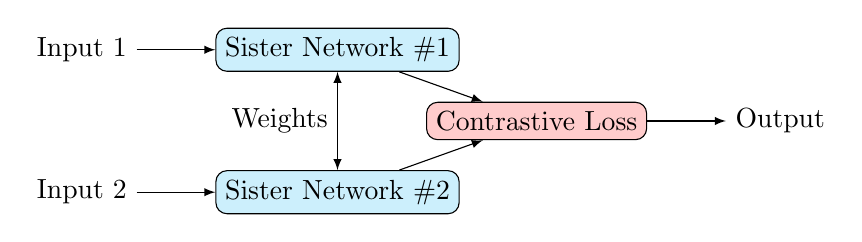
\begin{tikzpicture}
  \tikzstyle{module}=[rounded corners, draw]
  \tikzstyle{sister}=[module, fill=cyan!20]

  \node [sister] (S-1) at (0, 0) {Sister Network \#1};
  \node [below = .5 of S-1] (aux-1) {};
  \node [sister, below = .5 of aux-1] (S-2) {Sister Network \#2};

  \node [left = of S-1] (I-1) {Input 1};
  \node [left = of S-2] (I-2) {Input 2};

  \node [module, right = of aux-1, fill=red!20] (M-1) {Contrastive Loss};

  \node [right = of M-1] (O-1) {Output};

  \draw [-latex] (I-1) -- (S-1);
  \draw [-latex] (I-2) -- (S-2);

  \draw [-latex] (S-1) -- (M-1);
  \draw [-latex] (S-2) -- (M-1);

  \draw [-latex] (M-1) -- (O-1);

  \draw [latex-latex] (S-1) -- (S-2) node[midway, left] {Weights};
\end{tikzpicture}
  \caption{Siamese Network basic structure \label{fig:siamese}}
\end{figure}

The design is one of the most important parts of the project, since it will have a huge
impact in the final results. It will take around four weeks to complete and more or less
and it will be a trial and error process to try to see which architecture for the sister
network is best suited to solve the problem.

In this phase the designed networks will be very shallow to make small and fast improvements
since the training time could be an issue.

\subsubsection{Build deep siamese network}

Once a initial shallow network is already created then the next step will be to try an create
a more deep version, either using a pre-trained model or training a deep model from zero.

Using a pre-trained network will improve the development process since it will allow us
to make use of transfer learning and will have a low training time. However training the model
from zero may give us better results but although with the cost of spending too much time.
The deep network process should take two more weeks to complete.

\subsubsection{Compare the model against other ones}

Once the final deep model is created then it will be compared against different methods of 
survival analysis. Since this method will be the first one using both image data and scalar 
data it will be compared against models using only one or the other. 

The comparison will be against models using a Cox Proportional Hazards model using either
the \emph{radiomics} features extracted with \texttt{PyRadiomics} from CT scans or using 
directly the RAW image data extracted from the scans.

To do all this comparisons the same original data, the head and neck dataset, must be 
used so it may require running again the training process using the compared method. 
That's why it will take two weeks for this task to complete.

\subsection{Estimated time}

In \autoref{tab:time} an estimation of the number of hours dedicated to each task is shown.

\begin{table}[H]
  \centering{}
  \begin{tabular}{|l|r|}
    \hline
    Task & Estimated duration (h) \\ \hline \hline
    Acquire background in CNN & 120 \\ \hline
    Get familiar with survival models & 80 \\ \hline
    Preprocess data & 40 \\ \hline
    Build shallow siamese network & 200 \\ \hline
    Build deep siamese network & 80 \\ \hline
    Compare models & 80 \\ \hline
    Final stage & 160 \\ 

  
    \hline \hline
    \textbf{Total} & 760 \\
    \hline
  \end{tabular}
  \caption{Estimated time for each task \label{tab:time}}
\end{table}

\subsection{Gantt chart}

\autoref{fig:gantt} shows the planning of the different tasks of the project in a Gantt chart.

\begin{figure}[H]
  \centering{}
  \def\gantttext{4cm}
  \begin{ganttchart}[
      time slot format=isodate,
      x unit = .9mm,
      y unit title = 0.7cm,
      y unit chart = 0.5cm,
      group label font = \tiny\bf,
      title label font = \tiny,
      bar label font = \tiny,
      vgrid={*{4}{draw=none},dotted,*{2}{draw=none}},
      hgrid,
      calendar week text = {\startday},
      link bulge = 2,
    ]{2018-02-14}{2018-06-29}
    \gantttitlecalendar{month=shortname, week} \\


    % Start gantt itself
    \ganttgroup{Preamble}{2018-02-14}{2018-03-25} \\
    \ganttbar{Getting started}{2018-02-14}{2018-02-18} \\
    \ganttlinkedbar{Learn about CNN}{2018-02-19}{2018-03-11} \\
    \ganttlinkedbar{Learn about DeepSurv}{2018-03-12}{2018-03-25} \\

    
    \ganttgroup{Build siamese network}{2018-03-26}{2018-05-20} \\
    \ganttbar{Preprocess data}{2018-03-26}{2018-04-01} \\
    \ganttlinkedbar{Build shallow network}{2018-04-02}{2018-05-06} \\
    \ganttlinkedbar{Build deep network}{2018-05-07}{2018-05-20} \\

    \ganttgroup{\parbox[r]{2.3cm}{Compare models and extract conclusions}}{2018-05-21}
    {2018-06-03} \\

    \ganttbar{Compare models}{2018-05-21}{2018-05-27} \\
    \ganttlinkedbar{Extract conclusions}{2018-05-28}{2018-06-03} \\

    \ganttgroup{Final Stage}{2018-06-04}{2018-06-29} \\
    \ganttbar{Write final report}{2018-06-04}{2018-06-17} \\
    \ganttbar{End project}{2018-06-18}{2018-06-24} \\
    \ganttbar{Presentation}{2018-06-25}{2018-06-29} \\

  \end{ganttchart}
  \caption{Gantt chart of the project \label{fig:gantt}}
\end{figure}

\subsection{Alternatives and action plan}


\subsubsection{Complexity of the built model}

\subsubsection{Bugs}

\subsubsection{Unavailability of SharcNet}

\subsubsection{Training times}

% !TEX root = main.tex

% \addtocontents{toc}{\protect\newpage}
\secc{Design and implementation}

\ssecc{Get familiar with survival models}

\ssecc{Preprocess data}

As it was previously stated the data needs to be preprocessed before start training with it.
This steps are required because small changes can really help in reducing the time needed to
fit the model. Also, by normalizing the data and setting variance to 1 and mean to 0 the network
can converge faster.
~\cite{neural:efficient-backprop}

% TODO: Insert paper about batch normalization.

\sssecc{Image data}

The imaging data in the \Gls{PMHNK} contains 671 folders, each one with the scan of one patient. 
We also have the clinical information of 661 patients, although we do not have a \gls{CT} for
each of the clinical information patients. Through the intersection of each of the two data
sources we have 544 patients with both a \gls{CT} scan and the clinical information.

However, because there was a problem in the way the \gls{CT} scan was computed we only have
the tumour annotations for 509 of the 544 patients, so the data that we can use is reduced
again. \textbf{509} will be the final dataset size that will be used for the next 
steps.

For all the valid patients their directory structure is the same. For example if we have the
patient \texttt{FHBO003} 

Preprocessing the image data requires multiple steps:

\begin{enuerate}
  
\end{enuerate}

\sssecc{Scalar data}

\ssecc{Build shallow siamese network}

\ssecc{Build scalar only siamese network}

\ssecc{Build deeep siamese network}



\pagebreak

% \printglossary[type=\acronymtype]
\printglossaries

\addphantomsec{References}{\seccn}
\printbibliography[heading=none]{}

\end{document}